\documentclass{article}
\usepackage[utf8]{inputenc}
\usepackage[czech]{babel}
\usepackage[dvipsnames]{xcolor}

\usepackage{graphicx}
\usepackage{amsthm}
\usepackage{amsmath}
\def\baselinestretch{1}\normalsize 
\usepackage{wrapfig}
\usepackage{pgf,tikz} 
\usepackage{dsfont}

\usepackage[bottom]{footmisc}
\usepackage{footnote}
\usepackage{textcomp}
\usepackage{amssymb}
\usepackage{url}
\usepackage{float}
\usepackage{caption}
\usepackage{subcaption}
\usepackage{multirow}
\usepackage[total={17cm,25cm}, top=3cm, left=2.5cm, right=2.5cm, bottom = 2cm, includefoot]{geometry}
\usepackage{nicefrac}

\usepackage{braket}

\usepackage{centernot}
\usepackage{mathtools}

\newcommand{\incfig}[1]{%
    \def\svgwidth{\columnwidth}
    \import{./figures/}{#1-1.png_tex}
}


\begin{document}
\begin{center}
    \Large
    \textbf{Poznámky}
           
    \vspace{0.4cm}
    \small
    \textbf{24. září 2021}
\end{center}

\begin{section}{Rekapitulace}
Máme hamiltonián 
    $$\hat{H}_D = 
        (1 - \xi)\hat{n} - \frac{\xi}{N - 1} \hat{W}^2_D - \epsilon\hat{D_x},
    $$
kde změna parametru $\xi$ odpovídá přechodu mezi dvěma rovnovážnými polohami molekuly v řetízku a $\epsilon$
udává sílu poruchy (elmag. pole). Zajímají nás OTOCy různých kombinací operátorů. 

Podobným hamiltoniánem, sestaveným z operátorů tvořící stejnou algebru a podalgebry, lze popsat typ Bose-Einsteinova plazmatu. Místo 
kreace a anihilace vibronových stavů ve směrech x a y (resp. + a -) mluvíme o kreaci kladných a záporných bosonů v kondenzátu s celkovým
počtem N bosonů. 
\end{section}

\begin{section}{OTOCy}
    \begin{subsection}{Mikrokanonický OTOC}

    Zatím jsme OTOCy počítaly jako stopu přes celý operátor 
    $$ C(t) = \text{Tr}([W(t),V(0)]^{\dagger}[W(t),V(0)]).$$

    Implementovali jsme ještě výpočet mikrokanonických OTOCů. Mějme bázi
    $\{ \ket{n} \}$, mikrokanonický OTOC $c_n(t)$ je dán jako

    \begin{align*}c_n(t) &= \bra{n} [W(t),V(0)]^{\dagger}[W(t),V(0)] \ket{n} =
    \bra{n} [W(t),V(0)]^{\dagger} \sum_i \ket{i}\bra{i} [W(t),V(0)] \ket{n} \\
    &=\sum_i \bra{i} [W(t),V(0)] \ket{n} \bra{i} [W(t),V(0)] \ket{n}^{\dagger}
    \end{align*}


    \end{subsection}

    \begin{subsection}{Oscilace}

        Vzhledem k tomu, že by oscilace OTOCů mohly mít spojitost s chaosem, Fourierovou transformací převádíme
        mikrokanonické OTOCy na jednotlivé frekvence. Míru rozpliznutí OTOCU v prostoru frekvencí (v prostoru s diskrétními frekvencemi
        je reprezentován vektorem $\vec{c} = \sum_f a_f \vec{f}$) indikujeme 
        pomocí vztahu

        $$D(c) = \frac{\sum_f a_f^4}{(\vec{c}\cdot\vec{c})^2},$$

        kde jmenovatel slouží k normalizaci vektoru OTOCu. Pak platí $D(c) \in \langle 0, 1\rangle$, kde 
        0 odpovídá úplně delokalizovanému signálu (všechny frekvence jsou stejně zastoupeny) a 1 odpovídá signálu
        s jedinou frekvencí.

        Praktičtější by mohla být ještě transformovaná hodnota 
        $$\bar{D}(c) = \ln (D(c)^{-1}),$$
        u které platí $\bar{D}(c) \in \langle 0, \infty )$ - jde od úplně lokalizovaného k delokalizovanému signálu.

        Na následujících dvou obrázcích je ukázka. Jedná se o OTOC $[n(t),W^2(0)]$. V obou případech mikrokanonický OTOC 
        na 400. energetické hladině. 
    \end{subsection}

    \begin{figure}[H]
        \begin{center}
            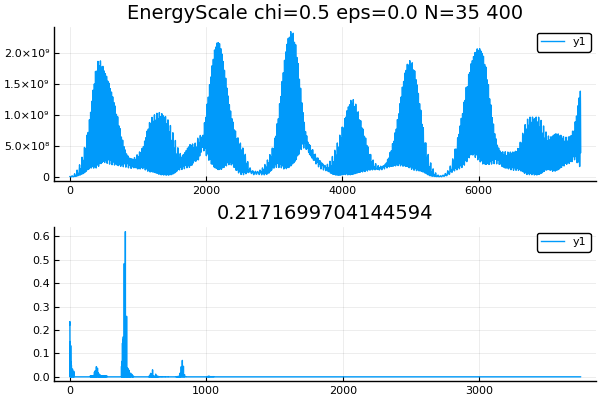
\includegraphics[width=12cm]{E_0.png}
        \end{center}
        
        \caption{Mikrokanonický OTOC $[n(t),W^2(0)]$ na 400. energetické hladině. Na horním grafu je mikrokanonický OTOC $c(t)$
         a na spodní je jeho Fourierova transformace (normovaná). Parametry jsou uvedeny nad prvním obrázkem ($\xi$ je špatně označeno jako 
         $chi$). Míra 
        $D(c)$ je uvedena nad druhým obrázkem.}
    \end{figure}

    \begin{figure}[H]
        \begin{center}
            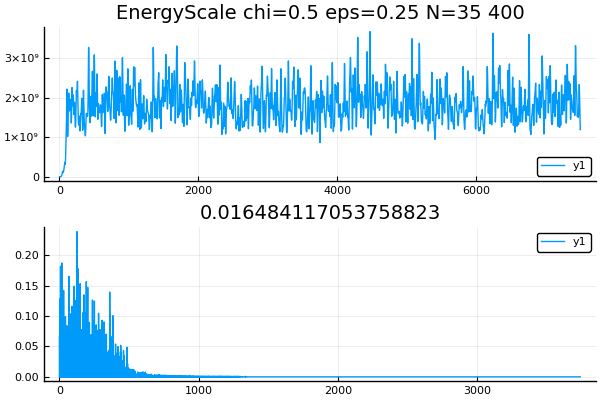
\includegraphics[width=12cm]{E_0.25.png}
        \end{center}
        
        \caption{Mikrokanonický OTOC $[n(t),W^2(0)]$ na 400. energetické hladině. Na horním grafu je mikrokanonický OTOC $c(t)$
        a na spodní je jeho Fourierova transformace (normovaná). Parametry jsou uvedeny nad prvním obrázkem. Míra 
        $D(c)$ je uvedena nad druhým obrázkem.}
    \end{figure}

    \subsection{Energetická závislost OTOCů}

    Energerickou závislost OTOCů jsme určovali pomocí dvou ukazatelů. Prvním je delokalizace
    ve frekvenční bázi $\bar{D}$ a druhým je střední hodnota (časová) a odchylka OTOCu v dlouhých časech (v následujících
    ukázkách děláme střední hodnotu z posledních 1000 bodů $c(t)$).

    Oba ukazatelé vykazují obecně zvláštní závisloti na energii a to sice výzarné oscilace.
    Vedlejší energetické hladiny vykazují často výrazný skok v těchto ukazatelích.  

    \begin{figure}[H]
        \centering
        \begin{subfigure}{.5\textwidth}
          \centering
          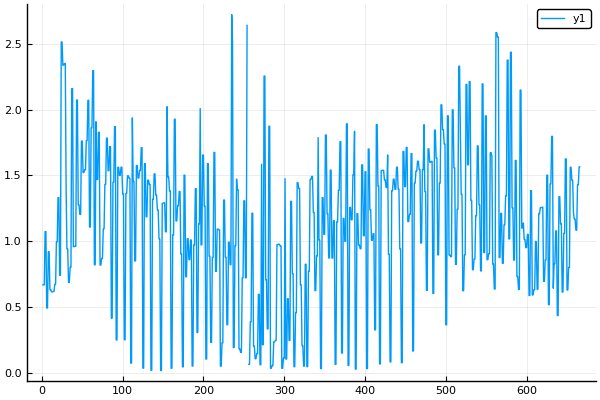
\includegraphics[width=1.0\linewidth]{Escale0.png}

        \end{subfigure}%

        \begin{subfigure}{.5\textwidth}
          \centering
          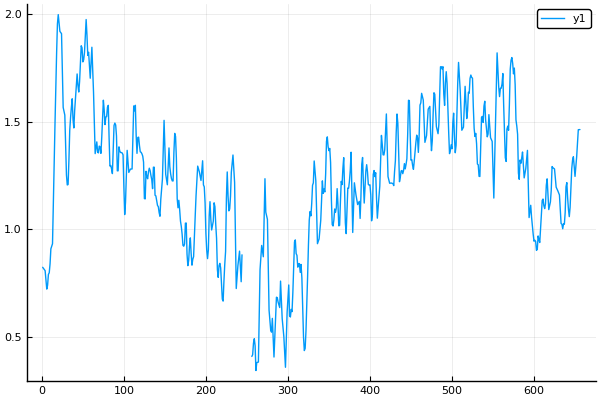
\includegraphics[width=1.0\linewidth]{Escale0smooth.png}

        \end{subfigure}
        \caption{Energetický závislost mikrokanonického OTOCu. Na ose x je pořadí hladin a na ose y je delokalizace OTOCu středovaného
        přes příslušnou hladinu ve frekvenční bázi $\bar{D}$. Parametry $\xi = 0.5, \epsilon = 0.0, N =35$. Na spodním grafu je zhlazení 
        přes deset bodů.}
        \end{figure}


        \begin{figure}[H]
            \centering
            \begin{subfigure}{.5\textwidth}
              \centering
              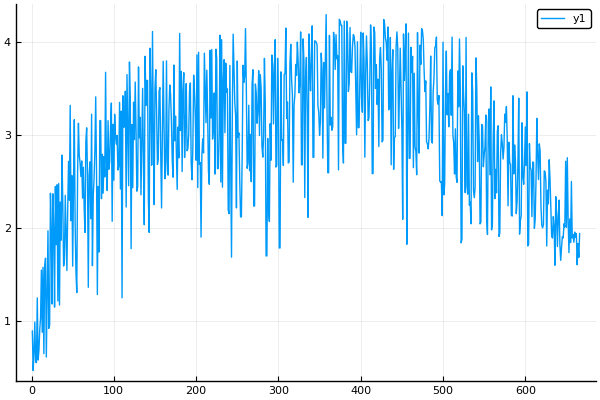
\includegraphics[width=1.0\linewidth]{Escale0.25.png}
    
            \end{subfigure}%
    
            \begin{subfigure}{.5\textwidth}
              \centering
              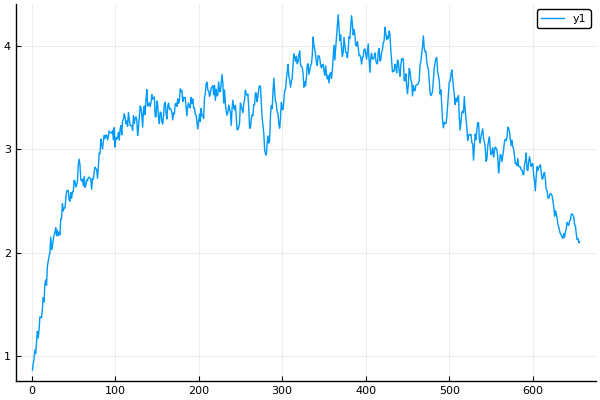
\includegraphics[width=1.0\linewidth]{Escale0.25smooth.png}
    
            \end{subfigure}
            \caption{Energetický závislost mikrokanonického OTOCu. Na ose x je pořadí hladin a na ose y je delokalizace OTOCu středovaného
            přes příslušnou hladinu ve frekvenční bázi $\bar{D}$. Parametry $\xi = 0.5, \epsilon = 0.25, N =35$. Na spodním grafu je zhlazení 
            přes deset bodů.}
            \end{figure}
  


            Ještě zajímavější závislost na energii vykazuje střední hodnota OTOCů v dlouhých časech. 


            \begin{figure}[H]
                \begin{center}
                    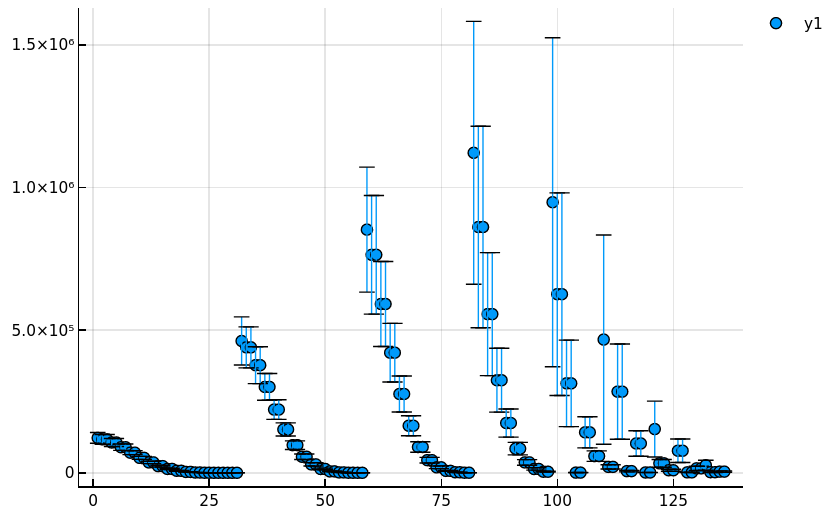
\includegraphics[width=12cm]{Mean 0.png}
                \end{center}
                
                \caption{Závislost střední hodnoty s odchylkou mikrokanonického 
                 OTOCu $[n(t),W^2(0)]$ na energii. Na ose x je pořadí hladiny. Parametry jsou $\xi = 0.75, \epsilon = 0.0, N = 15$}
            \end{figure}

            \begin{figure}[H]
                \begin{center}
                    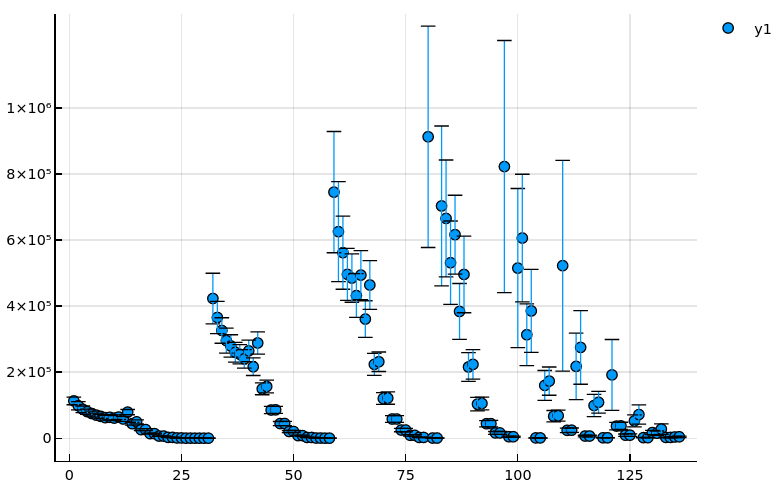
\includegraphics[width=12cm]{Mean 0.03.png}
                \end{center}
                
                \caption{Závislost střední hodnoty s odchylkou mikrokanonického 
                 OTOCu $[n(t),W^2(0)]$ na energii. Na ose x je pořadí hladiny. Parametry jsou $\xi = 0.75, \epsilon = 0.03, N = 15$}
            \end{figure}

            \begin{figure}[H]
                \begin{center}
                    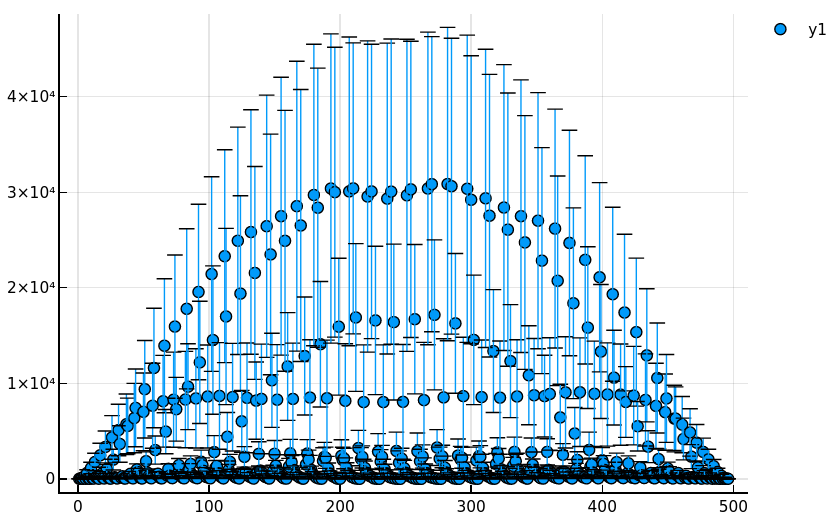
\includegraphics[width=12cm]{Mean 10.png}
                \end{center}
                
                \caption{Závislost střední hodnoty s odchylkou mikrokanonického 
                 OTOCu $[n(t),W^2(0)]$ na energii. Na ose x je pořadí hladiny. Parametry jsou $\xi = 0.75, \epsilon = 10.0, N = 15$}
            \end{figure}

            Obecně na grafech střední hodnoty OTOCů vidíme struktury, které na sebe přechází při změnách parametrů $\xi$ a $\epsilon$. 
            V krajních hodnotách parametrů vidíme pravidelné struktury (obr. 5 a 7), kterou jsou posunem parametrů narušovány.

            Vzhledem ke složitým obrazcům se energetická škála nezdá být vhodnou charakteristikou míry oscilací ani středních hodnot 
            OTOCů.

\subsection{Fockovská báze}

            Zkusíme mikrokanonické OTOCy počítat ve fockovské bázi $\{\ket{N,n_+,n_-}\}$, kde $n_+$ je počet vibronů 
            kreovaných operátorem $\tau_+$ a obdobně $n_-$. $N$ je celkový počet částic. Zajímavá je i interpretace pomocí 
            Bose-Einsteinova plazmatu, kde $n_+$ je počet kladných bosonů, $n_-$ záporných a $N$ je celkový počet 
            bosonů včetně těch neutrálních.

            Střední hodnoty mikrokanonických otoků ve fockovské bázi lze znázornit na heatmapě, kde na ose x je $n_+$
            a na ose y je $n_-$. Vzhledem k fixnímu počtu $N$ je tak zaplněna oblast (nenulové hodnoty) grafu jen pod diagonálou, jak bude 
            vidět na následujících grafech.

            Časové střední hodnoty a delokalizace $\bar{D}$ OTOCů z grafů na obrázcích 5 a 6 ve fockovské bázi jsou na 
            následujících grafech.


                \begin{figure}[H]
                    \begin{subfigure}{.5\textwidth}
                      \centering
                      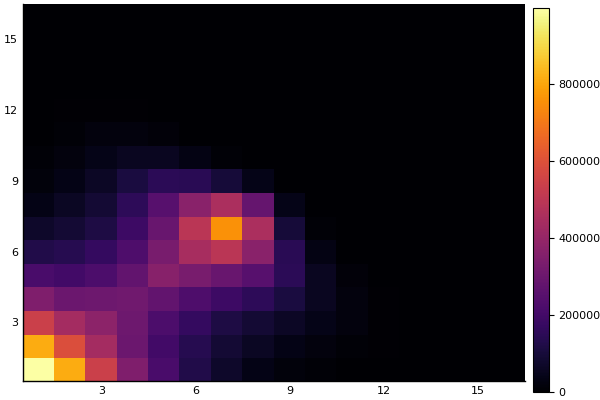
\includegraphics[width=1.0\linewidth]{HM0.png}
                     
                    \end{subfigure}%
                    \begin{subfigure}{.5\textwidth}
                      \centering
                      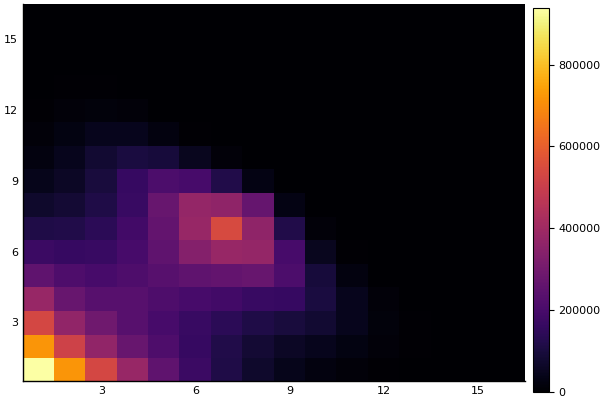
\includegraphics[width=1.0\linewidth]{HM0.03.png}
                      
                    \end{subfigure}
                    \caption{Časová střední hodnota mikrokanonických OTOCů ve fockovské bázi. Na ose x je počet kladných bosonů a na 
                    ose y je počet záporných bosonů. První graf je pro parametry $\xi = 0.75, \epsilon = 0.0, N = 15$.
                    Druhý graf je pro parametry $\xi = 0.75, \epsilon = 0.03, N = 15$}
                    \end{figure}

                    \begin{figure}[H]
                        \begin{subfigure}{.5\textwidth}
                          \centering
                          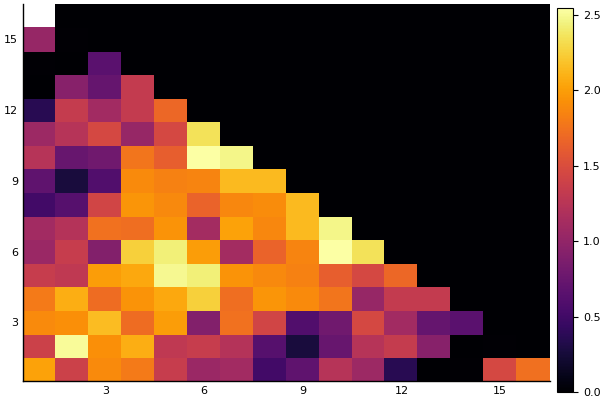
\includegraphics[width=1.0\linewidth]{HMD0.png}
                         
                        \end{subfigure}%
                        \begin{subfigure}{.5\textwidth}
                          \centering
                          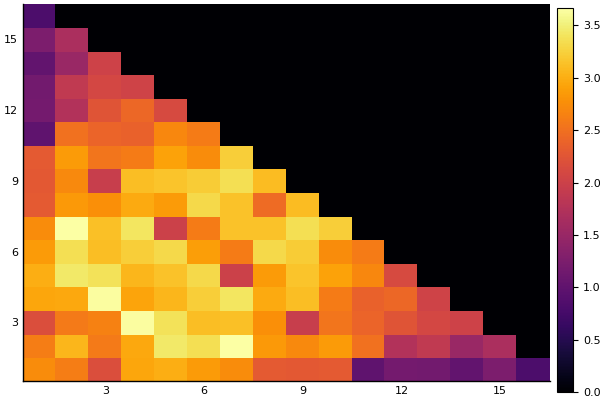
\includegraphics[width=1.0\linewidth]{HMD0.03.png}
                          
                        \end{subfigure}
                        \caption{Delokalizace $\bar{D}$ mikrokanonických OTOCů ve fockovské bázi. Na ose x je počet kladných bosonů a na 
                        ose y je počet záporných bosonů. První graf je pro parametry $\xi = 0.75, \epsilon = 0.0, N = 15$.
                        Druhý graf je pro parametry $\xi = 0.75, \epsilon = 0.03, N = 15$}
                        \end{figure}

            
                        Ve fockovské bázi vidíme lokalizované oblasti s vysokými a nízkými hodnotami obou ukazatelů. U některých 
                        OTOCů je to ještě výraznější. Na následujících grafech jsou výsledky z OTOCů $[\hat{n}_+(t),\hat{n}_+(0)]$.
                        Postupně zvyšujeme poruchu z $\epsilon = 0.0$ na $\epsilon = 0.05$ 

                        \begin{figure}[H]
                            \begin{subfigure}{.33\textwidth}
                              \centering
                              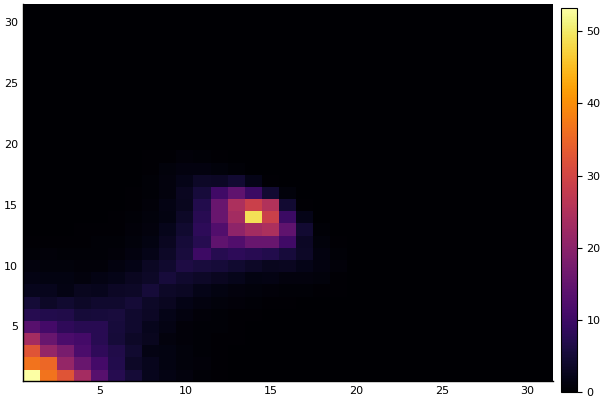
\includegraphics[width=1.0\linewidth]{1.png}
                              \caption{$\epsilon$ = 0.0}
                             
                            \end{subfigure}%
                            \begin{subfigure}{.33\textwidth}
                              \centering
                              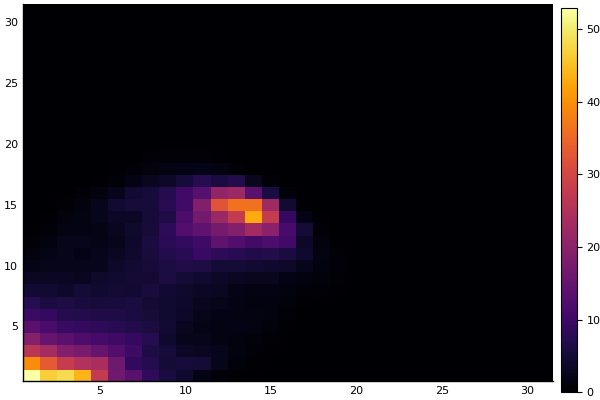
\includegraphics[width=1.0\linewidth]{2.png}
                              \caption{$\epsilon$ = 0.01}


                            \end{subfigure}%
                            \begin{subfigure}{.33\textwidth}
                              \centering
                              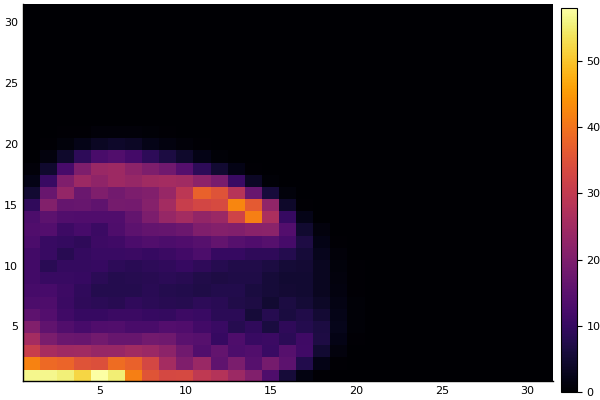
\includegraphics[width=1.0\linewidth]{3.png}
                              \caption{$\epsilon$ = 0.02}

                            \end{subfigure}%

                              \begin{subfigure}{.33\textwidth}
                                \centering
                                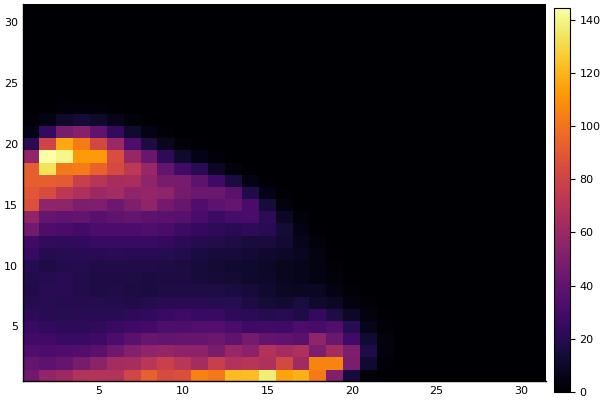
\includegraphics[width=1.0\linewidth]{4.png}
                              \caption{$\epsilon$ = 0.03}

                               
                              \end{subfigure}%
                              \begin{subfigure}{.33\textwidth}
                                \centering
                                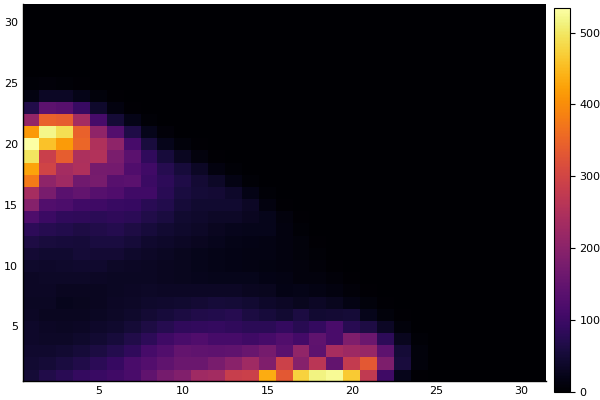
\includegraphics[width=1.0\linewidth]{5.png}
                              \caption{$\epsilon$ = 0.04}

  
                              \end{subfigure}%
                              \begin{subfigure}{.33\textwidth}
                                \centering
                                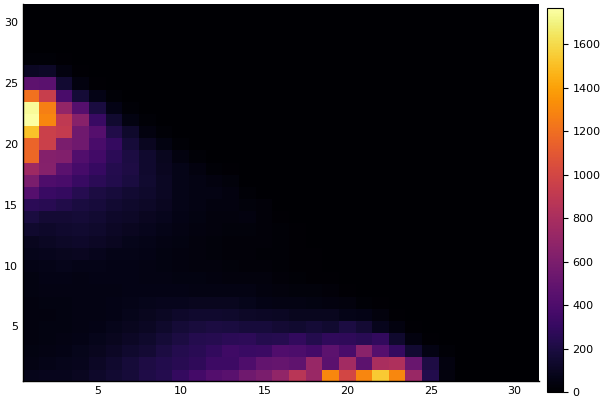
\includegraphics[width=1.0\linewidth]{6.png}
                              \caption{$\epsilon$ = 0.05}

                            \end{subfigure}


                            \caption{Časová střední hodnota mikrokanonických OTOCů ve fockovské bázi. Na ose x je počet kladných bosonů a na 
                            ose y je počet záporných bosonů. Parametry $\xi = 0.75, \epsilon = 0.0 - 0.05, N = 30$.}
                            \end{figure}

                            Vidíme, že se maxima časových středních hodnot po grafu přímo pohybují v závislosti na síle poruchy. 


                            \begin{figure}[H]
                                \begin{subfigure}{.33\textwidth}
                                  \centering
                                  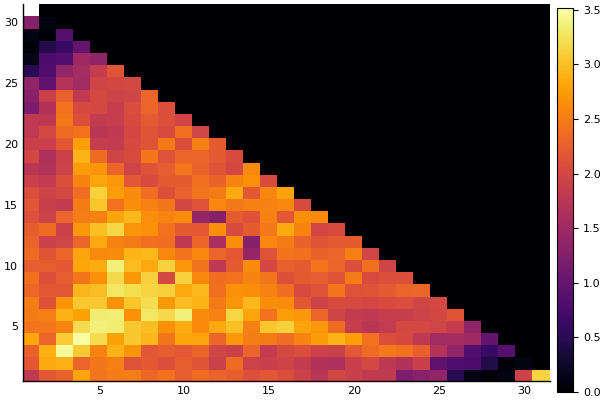
\includegraphics[width=1.0\linewidth]{HM1.png}
                                  \caption{$\epsilon$ = 0.0}
                                 
                                \end{subfigure}%
                                \begin{subfigure}{.33\textwidth}
                                  \centering
                                  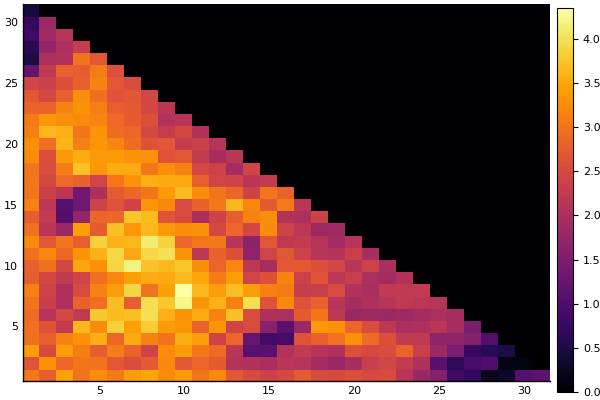
\includegraphics[width=1.0\linewidth]{HM2.png}
                                  \caption{$\epsilon$ = 0.01}
    
    
                                \end{subfigure}%
                                \begin{subfigure}{.33\textwidth}
                                  \centering
                                  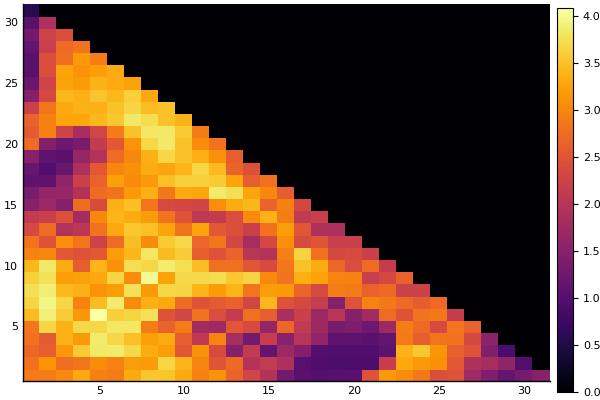
\includegraphics[width=1.0\linewidth]{HM3.png}
                                  \caption{$\epsilon$ = 0.02}
    
                                \end{subfigure}%
    
                                  \begin{subfigure}{.33\textwidth}
                                    \centering
                                    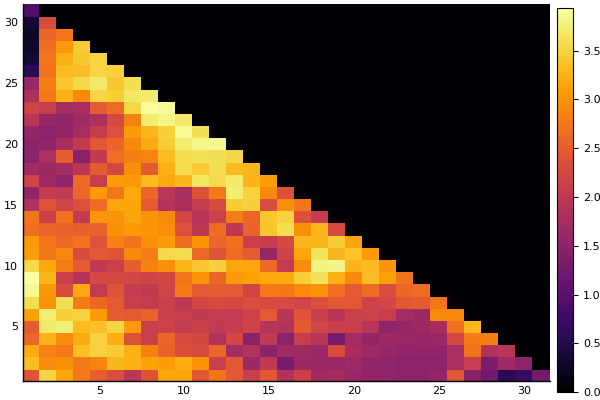
\includegraphics[width=1.0\linewidth]{HM4.png}
                                  \caption{$\epsilon$ = 0.03}
    
                                   
                                  \end{subfigure}%
                                  \begin{subfigure}{.33\textwidth}
                                    \centering
                                    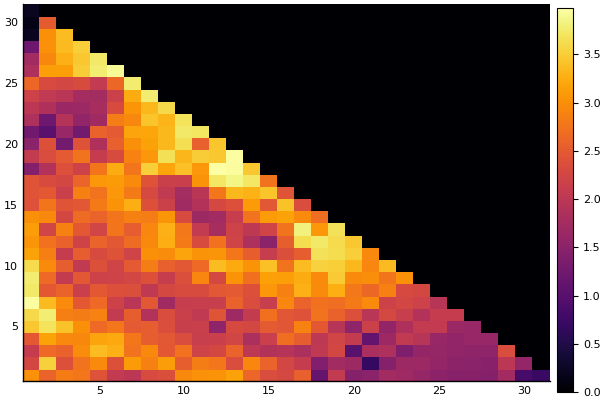
\includegraphics[width=1.0\linewidth]{HM5.png}
                                  \caption{$\epsilon$ = 0.04}
    
      
                                  \end{subfigure}%
                                  \begin{subfigure}{.33\textwidth}
                                    \centering
                                    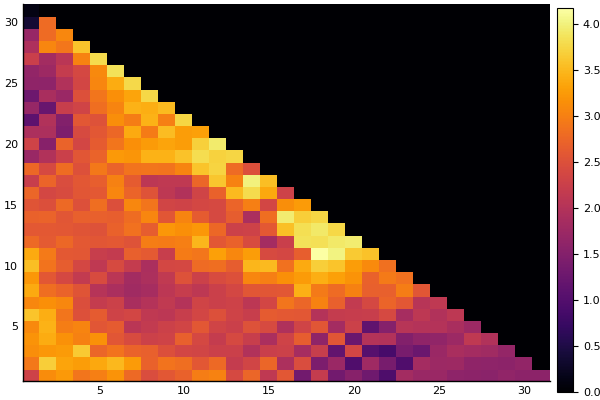
\includegraphics[width=1.0\linewidth]{HM6.png}
                                  \caption{$\epsilon$ = 0.05}
    
                                \end{subfigure}
    
    
                                \caption{Delokalizace mikrokanonických OTOCů ve fockovské bázi. Na ose x je počet kladných bosonů a na 
                                ose y je počet záporných bosonů. Parametry $\xi = 0.75, \epsilon = 0.0 - 0.05, N = 30$.}
                                \end{figure}


                                Zdá se, že OTOCy různých skupin operátorů (operátory počtů částic, operátory D, operátory P a Q) 
                                se liší právě v podobě heatmap použitých indikátorů. Je to zatím jen vágní představa, ale různým
                                skupinám zdá se odpovídají různé obrazce na heatmapách, u kterých vidíme buď pohyb maxim jako 
                                v předchozích grafech, nebo rozplývání jako na následujících grafech časových středních hodnot
                                OTOCů operátorů $[n(t),W^2(0)]$. 


                                \begin{figure}[H]
                                    \begin{subfigure}{.33\textwidth}
                                      \centering
                                      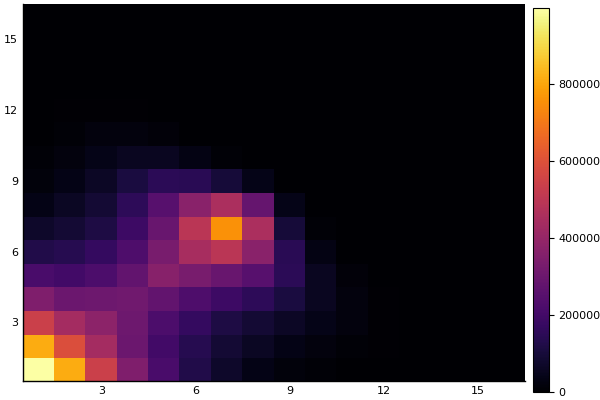
\includegraphics[width=1.0\linewidth]{nW0.png}
                                      \caption{$\epsilon$ = 0.0}
                                     
                                    \end{subfigure}%
                                    \begin{subfigure}{.33\textwidth}
                                      \centering
                                      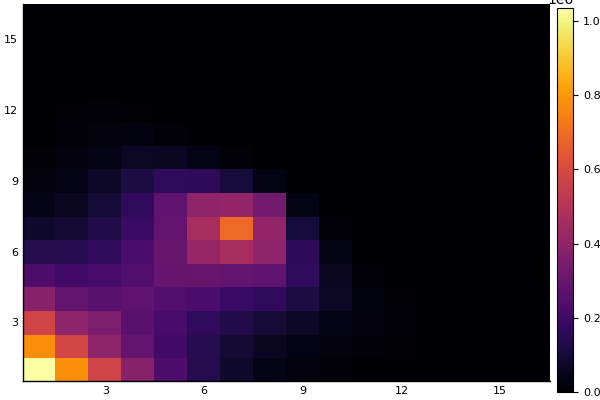
\includegraphics[width=1.0\linewidth]{nW0.01.png}
                                      \caption{$\epsilon$ = 0.01}
        
        
                                    \end{subfigure}%
                                    \begin{subfigure}{.33\textwidth}
                                      \centering
                                      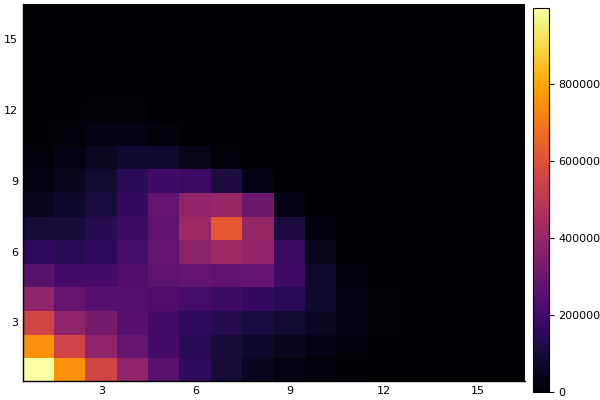
\includegraphics[width=1.0\linewidth]{nW0.02.png}
                                      \caption{$\epsilon$ = 0.02}
                                    \end{subfigure}%
        
                                      \begin{subfigure}{.33\textwidth}
                                        \centering
                                        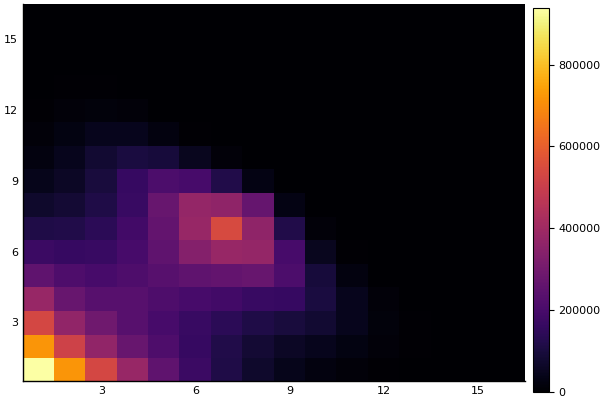
\includegraphics[width=1.0\linewidth]{nW0.03.png}
                                      \caption{$\epsilon$ = 0.03}
                                      \end{subfigure}%
                                      \begin{subfigure}{.33\textwidth}
                                        \centering
                                        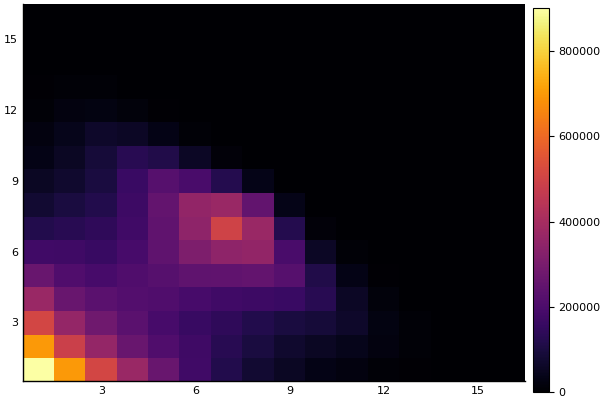
\includegraphics[width=1.0\linewidth]{nW0.04.png}
                                      \caption{$\epsilon$ = 0.04}
                                      \end{subfigure}%
                                      \begin{subfigure}{.33\textwidth}
                                        \centering
                                        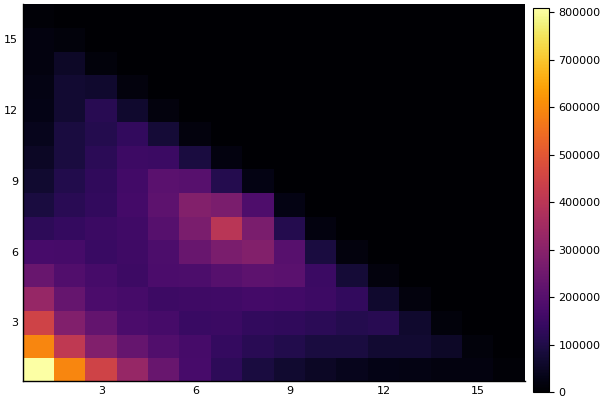
\includegraphics[width=1.0\linewidth]{nW0.1.png}
                                      \caption{$\epsilon$ = 0.1}
                                    \end{subfigure}%

                                      \begin{subfigure}{.33\textwidth}
                                        \centering
                                        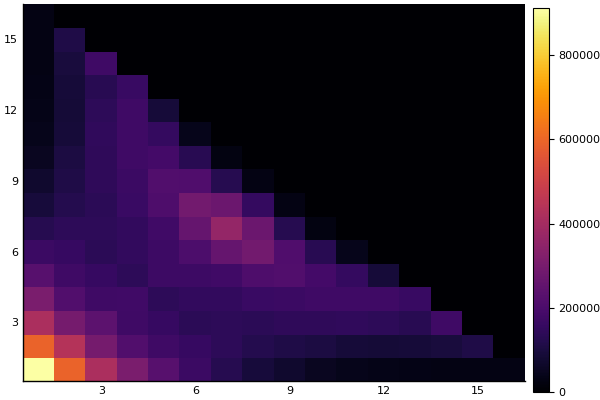
\includegraphics[width=1.0\linewidth]{nW0.2.png}
                                      \caption{$\epsilon$ = 0.2}
                                      \end{subfigure}%
                                      \begin{subfigure}{.33\textwidth}
                                        \centering
                                        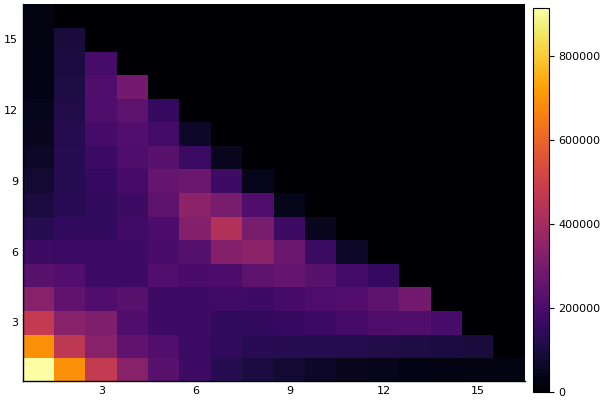
\includegraphics[width=1.0\linewidth]{nW0.3.png}
                                      \caption{$\epsilon$ = 0.3}
                                    \end{subfigure}%        
                                      \begin{subfigure}{.33\textwidth}
                                        \centering
                                        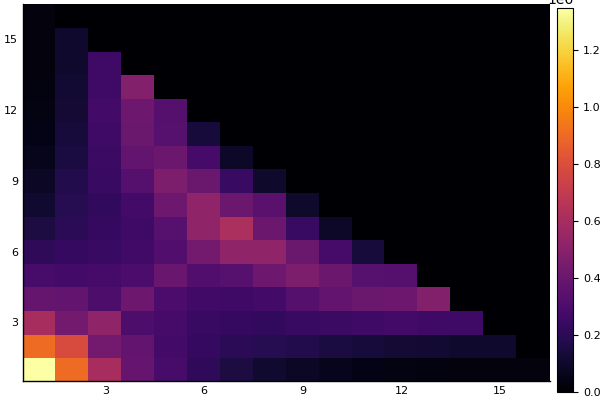
\includegraphics[width=1.0\linewidth]{nW0.4.png}
                                      \caption{$\epsilon$ = 0.4}
                                      \end{subfigure}

                                      \begin{subfigure}{.33\textwidth}
                                        \centering
                                        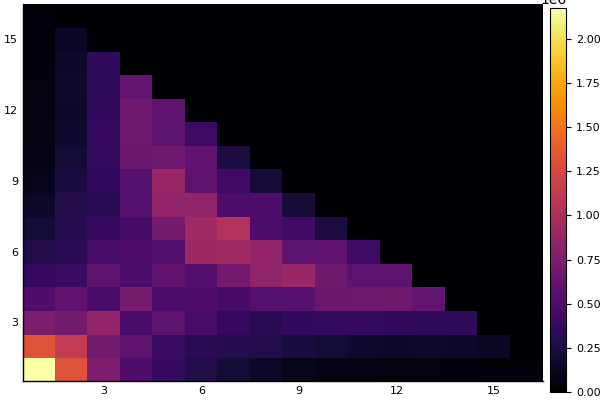
\includegraphics[width=1.0\linewidth]{nW0.5.png}
                                      \caption{$\epsilon$ = 0.5}
                 
                                      \end{subfigure}%
                                   

        
        
                                    \caption{Časová střední hodnota mikrokanonických OTOCů $[n(t),W^2(0)]$ ve fockovské bázi. Na ose x je počet kladných bosonů a na 
                                    ose y je počet záporných bosonů. Parametry $\xi = 0.75, \epsilon = 0.0 - 0.5, N = 15$.}
                                    \end{figure}

\end{section}


     \end{document}
